\documentclass[12pt]{article}


\usepackage[english]{babel}

% Set page size and margins
% Replace `letterpaper' with `a4paper' for UK/EU standard size
\usepackage[a4paper,top=2cm,bottom=2cm,left=3cm,right=3cm,marginparwidth=1.75cm]{geometry}
\newcommand\myemail[3]{%                %\newcommand\tpj@compose@mailto[3]{%
\edef\@tempa{mailto:#1?subject=#2 }%
\edef\@tempb{\expandafter\html@spaces\@tempa\@empty}%
\href{\@tempb}{#3}}
\usepackage[dvipsnames]{xcolor}
\definecolor{myblue}{RGB}{74, 144, 226}
\definecolor{myred}{RGB}{255, 2, 27}
%%%%%%%%%%%%%% Packages %%%%%%%%%%%%%%%%
\newtheorem{lemma}{Lemma}
%\usepackage{hyperref}
%\usepackage[...]{hyperref}
%\usepackage[colorlinks=true, allcolors=blue]{hyperref}
\usepackage[english]{babel}
\usepackage{amssymb}
\usepackage{underscore}
\usepackage{graphicx}
\usepackage{empheq}
\usepackage{booktabs}
\usepackage{tikz}
\newcommand*{\vertbar}{\rule[-1ex]{0.5pt}{2.5ex}}
\newcommand*{\horzbar}{\rule[.5ex]{2.5ex}{0.5pt}}
%% Some imports:
%\let\proof\relax
%\let\endproof\relax
%\let\example\relax
%\let\endexample\relax

%\usepackage{import}
\usepackage{float}
\usepackage{multirow}
\usepackage{amsmath}
% ,amsfonts,amssymb,amsthm
%\usepackage{subfigure}

\usepackage[ruled]{algorithm2e}
\usepackage{mathtools}
\usepackage[super]{nth}
\usepackage{caption}
\usepackage{subcaption}
\usepackage{graphicx}
%\usepackage{wrapfig}
\usepackage{verbatim} % comments
%\usepackage{comment}
%\renewenvironment{comment}{}{}
\usepackage{array}
\usepackage{supertabular}
\usepackage{longtable}
\usepackage{tabularx}
\usepackage{multirow}
\usepackage{colortbl}
\usepackage{fancyhdr}
%\usepackage{tcolorbox}
%\usepackage{tikz}
%\usetikzlibrary{math} %needed tikz library
%\usepackage[linesnumbered,ruled]{algorithm2e}
%\usepackage{pgf}
%\usepackage{pgfplots, pgfplotstable}
%\usetikzlibrary{fit,calc,positioning,decorations.pathreplacing,matrix}
%\usetikzlibrary{arrows}
%\usetikzlibrary{shapes}
%\usetikzlibrary{chains}
% Vector Styles
%\tikzstyle{load}   = [ultra thick,-latex]
%\tikzstyle{stress} = [-latex]
%\tikzstyle{dim}    = [latex-latex]
%\tikzstyle{axis}   = [-latex,black]
%\usepackage{pgffor}

%\usepackage{multido}
%\usepackage{calc}
%\usepackage{fp}
%\usepackage{xifthen}
%\usepackage{xargs}
\usepackage{etoolbox}
\DeclareMathAlphabet{\mathpzc}{OT1}{pzc}{m}{it}
\usepackage{breakcites} 
\usepackage[utf8]{inputenc}
\usepackage{helvet}
%\usepackage{geometry}
%\geometry{left=16mm, top=30mm, right=16mm, bottom=30mm}

%\usepackage{amssymb}
\usepackage{enumitem}
\usepackage{tabularx}
%\usepackage{xcolor}
\usepackage[absolute,overlay]{textpos}
%\usepackage{graphicx}
\usepackage{lipsum}
%\usepackage{caption}
\usepackage{multicol}
\usepackage{afterpage}
\usepackage{setspace}
\usepackage{parskip}
\usepackage{import} 
\usepackage[colorlinks=true,linkcolor=blue,allcolors=blue]{hyperref}%
\usepackage{hhline}
\graphicspath{{../figures/}}
%allcolors=blue

%%%%%%%%%%%%%% end Packages %%%%%%%%%%%%%%%%

%\pgfplotsset{compat=1.18}


\import{./}{Notations}

%\setlength{\parindent}{0cm}
%\noindent




\title{Rank Reduction Autoencoders - Enhancing interpolation on nonlinear manifolds.}
\author{Jad Mounayer$^{1,2,*}$, Sebastian Rodriguez$^{1,3}$, Chady Ghnatios$^{1,2}$, \\Charbel Farhat$^{4}$, Francisco Chinesta$^{1,5,6,7}$ \\ \\
$^1$PIMM, ENSAM Institute of Technology, 151 Boulevard de \\ l'Hôpital, 75013, Paris, France.\\
$^2$ PIMM Lab, SKF
Research Chair, Arts et Metiers
Institute of \\ Technology, Paris,
France\\
$^3$ESI Group Chair, PIMM, ENSAM Institute of Technology, \\ 151 Boulevard de l'Hôpital, 75013, Paris, France. \\
$^4$ Stanford University, Department of Aeronautics and Astronautics \\ Department of Mechanical Engineering and Industrial for \\ Computational and  Mathematical Engineering, \\ 496 Lomita Mall, Stanford, 94305, CA, USA. \\
$^5$RTE
Research Chair, PIMM, ENSAM Institute of Technology, \\ 151 Boulevard de l'Hôpital, 75013, Paris, France.\\
$^6$ CNRS@CREATE, 1 Create Way, \\ 04-05 Create Tower, Singapore, 138602, Singapore.\\
}



\begin{document}


\maketitle

\begin{abstract}
    Auteoncdoers encounter some limits as interpolators. If the latent space becomes too reduced, feature extraction can be done but their interpolation capabilities are limited to some parts of the parametric space. On the other hand, increasing the dimension of the latent space doesn't lead to any reduction, and hence doesn't help with interpolation. In this paper, we present Rank Reduction Autoencoders (RRAEs), Autoencoders that enforce large latent spaces to enable a linear reduction. We propose two formulations, a strong and a weak one, that enforce the latent space to have a low rank by constructing its reduced basis. We show that both formulations can interpolate efficiently between curves defining high-rank matrices, where the Vanilla Autoencoder fails. Further, we illustrate how preceeding RRAEs by a POD allows us to filter noisy data and reduce computational overhead. We finally show that both formulations can find an approximation of the intrinsic dimension of the parametric space if it is unknown in advance.
\end{abstract}
\textit{Keywords}: Rank Reduction, Autoencoders, Non-linear interpolation, Low-rank latent space, Non-linear model-order reduction, Singular Value Decomposition.

\section{Introduction}\label{sec:intro}
Interpolation over a parametric space is a widely considered topic in the literature since good interpolation allows us to reconstruct the solution of a physical problem in an entire parametric space from a few samples. Multiple techniques have been proposed to perform interpolation, mainly the Proper Orthogonal Decomposition with Interpolation (PODI) \cite{tezzele2019shape, nguyen2022efficient, rama2020towards}, or the sparse PGD (sPGD) \cite{chinesta2011short, sancarlos2023regularized}. Most of these techniques are based on Model Order Reductions, such as the Proper Orthogonal Decomposition (POD) \cite{rowley2004model, kerschen2005method}, the Proper Generalized Decomposition (PGD) \cite{ladeveze1985famille,rodriguez2019non, chinesta2014pgd}, and the Principal Component Analysis (PCA) \cite{labrin2020principal, gonzalez2018kpca}. These techniques depend on the fact that the solution can be represented by only a few parameters. In other words, if we stack multiple solutions into a matrix, only a few singular values of the matrix are dominant compared to the others (i.e. a low-rank matrix). When this assumption does not apply, the just referred techniques fail to create an efficient surrogate for the correct prediction of physical phenomena. Other techniques based on different formulations such as the Optimal Transport (OT) \cite{TORREGROSA202212, TORREGROSA202236} are also unable to interpolate properly in those settings. The efficiency of the methods presented above, as well as every low-rank technique (e.g. \cite{srebro2003weighted, liu2012robust, udell2016generalized, davenport2016overview}), drops when the solution is of a high rank.

On the other hand, machine learning algorithms are being used in almost every field due to their fast evaluations and their ability to approximate nonlinear behavior. This encouraged researchers to use them for data reduction and interpolation \cite{berrada2020training, rigol2001artificial}. One of the main architectures that are successful in feature recognition is Autoencoders \cite{hinton1993autoencoders}. By using Neural Networks as their encoding and decoding functions, Autoencoders with reduced latent spaces have been successfully used in many applications such as speech recognition \cite{vachhani2017deep, feng2014speech}, medical applications \cite{deng2019towards}, robotics \cite{park2018multimodal}, and others \cite{bank2023autoencoders}. However, Vanilla Autoencoders can only interpolate on a small part of the parametric domain and hence their use for interpolation is limited. This led to multiple enhancements such as Variational \cite{doersch2016tutorial}, or Sparse Autoencoders \cite{ng2011sparse} which improved Atueoncoders overall but did not definitively solve the interpolation issues.

Recently, the Implicit Rank-Minimizing Autoencoder (IRMAE) \cite{jing2020implicit}, and the Low-Rank Autoencoder (LoRAE) \cite{mazumder2023learning} showcased how increasing the latent space dimension while enforcing a low-rank achieves better results, including interpolation. Their models consist of adding one or more linear layers for the encoder to allow the Neural Network to find a latent space of a lower rank. The present paper proves that long latent spaces with low-rank can be exploited further.

Based on both the Koopman theory \cite{brunton2021modern} and the kPCA \cite{kpca}, it is known that we can find a linear behavior in larger spaces.  Inspired by these, we present Rank Reduction Autoencoders (RRAEs), which have large latent spaces that can be represented by a reduced basis. By enforcing the latent space to accept a linear reduction (hence a lower rank), we show that we end up with more powerful Autoencoders. Furthermore, since we find a reduced basis of the latent space, we can interpolate much more efficiently. In a certain sense, our proposal can be viewed as a kernel-free nonlinear PCA, overperforming usual kPCA techniques.

Our architecture includes two proposed formulations: a strong and a weak one. Throughout the paper, we show that the strong formulation finds orthogonal basis vectors and forms a POD-like basis, while the weak formulation is allowed to find non-orthogonal ones. We show that both formulations can interpolate efficiently between high-rank solutions where the Vanilla Autoencoder fails.

The present paper is structured as follows: section \ref{sec:HT} presents the architecture and both formulations proposed. Next, we explain our interpolation strategy in section \ref{sec:interp}. Section \ref{sec:insights} discusses why RRAEs can be more efficient than Vanilla AEs based on two examples. Then, we compare the interpolation capabilities of RRAEs with Vanilla AEs on a variety of problems in section \ref{sec:Nuemrical}. Finally, we summarize our work in Section \ref{sec:conclusions}.

Our results show that RRAEs perform much better with interpolation and that combining them with a POD can filter noise and reduce the computational overhead. Further, RRAEs can find an approximation of the intrinsic dimension of the parametric space if it is unknown in advance.
\section{Rank Reduction Autoencoders (RRAEs)}\label{sec:HT}
To define the architecture of RRAEs, we begin by defining autoencoder notations.

Let $\{X_i\}_{i\in [1, D]} \in \mathbb{R}^T$ be a set of $D$ series of observations, each of length $T$. We define our input $X\in \mathbb{R}^{T\times D}$ with $X_i$ as its $i$th column. Let, $Y \in \mathbb{R}^{L\times D}$ with $L$, the chosen dimension of the latent space. We also define the encoding map $e: \mathbb{R}^{T\times D} \xrightarrow{} \mathbb{R}^{L\times D}$ and the decoding map $d: \mathbb{R}^{L\times D} \xrightarrow{} \mathbb{R}^{T\times D}$. The Vanilla autoencoder can be written as the following two operations,
\begin{equation}
    Y = e(X), \qquad \tilde{X} = d(Y).
\end{equation}
In practice, we usually enforce that the output of the autoencoder gives us back the original data, hence the loss usually reads,
\begin{equation}
    \mathcal{L}(X, \tilde{X}) = \Vert X-\Tilde{X}\Vert_2, \quad \text{where,} \quad \Vert \cdot\Vert_2 \text{ is the L2-norm}.
\end{equation}
The idea behind RRAEs is to enforce the latent matrix to have a low rank while finding a reduced basis. In other words, let $Y = U^y\Sigma^yV^y$ be the Singular Value Decomposition (SVD) \cite{stewart1993early, nakatsukasa2017accuracy} of Y, and let $\{\sigma^y_i\}_{i \in [1, r]}$ be the sorted diagonal values of $\Sigma^y$, $r$ being the rank of Y. We want the following,
\begin{equation}\label{eqn:trunc}
    Y = \sum_{i=1}^r\sigma^y_iU^y_i(V^y)_i^T \qquad\Rightarrow\qquad Y\approx \sum_{i=1}^k\sigma^y_iU^y_i(V^y)_i^T, \qquad k\ll r,
\end{equation}
where $U^y_i$ is the $i$th column of $U^y$ and $(V^y)_i^T$ is the $i$th row of $V^y$. In other words, we can write $Y_d$, the $d$th column of $Y$ as,
\begin{equation}\label{eqn:alphas}
    Y_d = \sum_{i=1}^k\sigma^y_iU^y_i(V^y)_{i,d} = \sum_{i=1}^k\alpha^y_{i,d}U_i^y, \qquad\quad \forall d \in [1, D],
\end{equation}
with $(V^y)_{i,d}$ being entry $d$ of vector $(V^y_i)^T$.

Accordingly, for $k$ modes, each column of $Y$ is defined by $k$ coefficients and $k$ vectors. Further, vectors $U_i^y$ form a basis for the latent space. We can write \eqref{eqn:alphas} in matrix form as follows,
\begin{equation}\label{eqn:mat_form}
    Y = UA, \qquad \text{with: } A_{i,j}=\alpha_{i,j}^y, \quad U \in \mathbb{R}^{L\times k}. \quad A \in \mathbb{R}^{k\times D},
\end{equation}
Based on \eqref{eqn:alphas}, and \eqref{eqn:mat_form}, we propose two formulations that enforce the low rank of the latent space and find its reduced basis. The architecture is sketched in figure \ref{fig:mdoel_arch}.
\tikzset{every picture/.style={line width=0.75pt}} %set default line width to 0.75pt  
\begin{figure}



    \tikzset{every picture/.style={line width=0.75pt}} %set default line width to 0.75pt        

    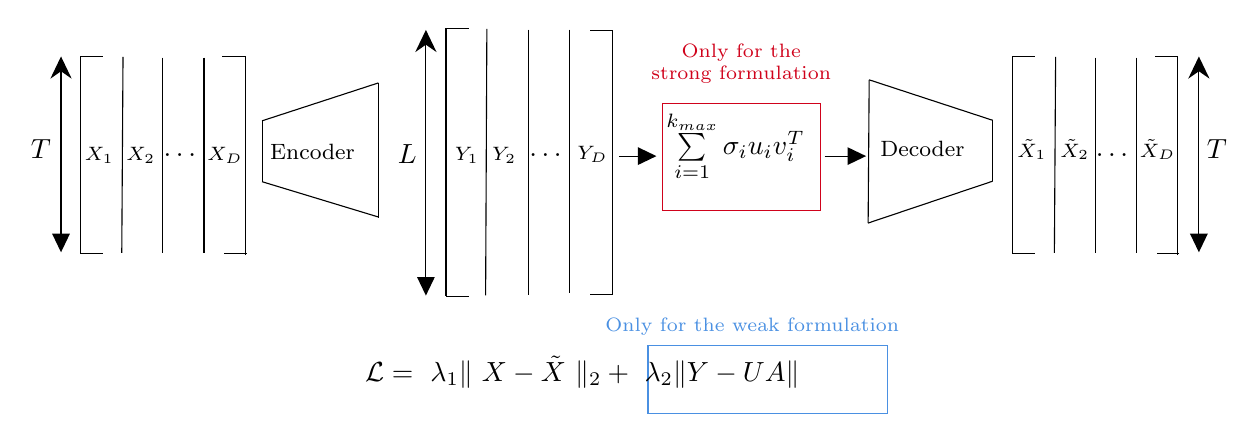
\begin{tikzpicture}[x=0.75pt,y=0.75pt,yscale=-1,xscale=1]
        %uncomment if require: \path (0,329); %set diagram left start at 0, and has height of 329

        %Straight Lines [id:da21499615368111846] 
        \draw    (37,108.56) -- (37,203.67) ;
        %Straight Lines [id:da16326946357296768] 
        \draw    (37,108.56) -- (47.89,108.56) ;
        %Straight Lines [id:da16265931324232152] 
        \draw    (37,203.67) -- (47.89,203.67) ;
        %Straight Lines [id:da5083389594267504] 
        \draw    (116.56,204.33) -- (116.56,108.67) ;
        %Straight Lines [id:da3615318503641125] 
        \draw    (117.22,203.7) -- (106.33,203.7) ;
        %Straight Lines [id:da9354769223516279] 
        \draw    (116.22,108.6) -- (105.33,108.6) ;
        %Straight Lines [id:da9284204806788381] 
        \draw    (57.67,108.87) -- (57.07,203.27) ;
        %Straight Lines [id:da9687380676381745] 
        \draw    (76.67,109.25) -- (76.67,203.25) ;
        %Straight Lines [id:da30039595434321] 
        \draw    (96.67,109.25) -- (96.67,203.25) ;
        %Straight Lines [id:da782396384119824] 
        \draw    (124.67,139.67) -- (180.67,121.42) ;
        %Straight Lines [id:da9238744798761502] 
        \draw    (124.67,169) -- (180.67,186) ;
        %Straight Lines [id:da44599235940336523] 
        \draw    (180.67,121.42) -- (180.67,186.33) ;
        %Straight Lines [id:da6964885949042201] 
        \draw    (213.3,95.06) -- (213.3,224.17) ;
        %Straight Lines [id:da06959562543054565] 
        \draw    (213.3,95.06) -- (224.19,95.06) ;
        %Straight Lines [id:da030633764479459424] 
        \draw    (213.3,224.17) -- (224.19,224.17) ;
        %Straight Lines [id:da3263511981591738] 
        \draw    (293.52,223.5) -- (293.52,96.17) ;
        %Straight Lines [id:da40502884422960217] 
        \draw    (293.52,223.5) -- (282.63,223.5) ;
        %Straight Lines [id:da8961788198500589] 
        \draw    (293.52,96.3) -- (282.63,96.3) ;
        %Straight Lines [id:da9774520960600939] 
        \draw    (232.97,95.37) -- (232.37,223.77) ;
        %Straight Lines [id:da5075505519042733] 
        \draw    (252.97,95.75) -- (252.97,223.75) ;
        %Straight Lines [id:da21045855349115494] 
        \draw    (272.97,95.75) -- (272.97,222.75) ;
        %Straight Lines [id:da754710144489299] 
        \draw    (124.67,139.67) -- (124.67,169) ;
        %Straight Lines [id:da7099185888654047] 
        \draw    (417.17,119.92) -- (476.67,139.42) ;
        %Straight Lines [id:da66143724081499] 
        \draw    (476.67,168.75) -- (416.67,188.92) ;
        %Straight Lines [id:da31064466545771574] 
        \draw    (417.17,119.92) -- (416.67,188.92) ;
        %Straight Lines [id:da5393972903258972] 
        \draw    (476.67,139.42) -- (476.67,168.75) ;
        %Straight Lines [id:da022156106633165695] 
        \draw    (296.67,156.67) -- (311.67,156.67) ;
        \draw [shift={(314.67,156.67)}, rotate = 180] [fill={rgb, 255:red, 0; green, 0; blue, 0 }  ][line width=0.08]  [draw opacity=0] (8.93,-4.29) -- (0,0) -- (8.93,4.29) -- cycle    ;
        %Straight Lines [id:da38115442380124565] 
        \draw    (395.67,156.67) -- (410.67,156.67) ;
        \draw [shift={(415.67,156.67)}, rotate = 180] [fill={rgb, 255:red, 0; green, 0; blue, 0 }  ][line width=0.08]  [draw opacity=0] (8.93,-4.29) -- (0,0) -- (8.93,4.29) -- cycle    ;
        %Shape: Rectangle [id:dp7709069667907207] 
        \draw  [color={rgb, 255:red, 208; green, 2; blue, 27 }  ,draw opacity=1 ] (317.4,131.47) -- (393.67,131.47) -- (393.67,182.67) -- (317.4,182.67) -- cycle ;
        %Shape: Rectangle [id:dp24666081940562967] 
        \draw  [color={rgb, 255:red, 74; green, 144; blue, 226 }  ,draw opacity=1 ] (310.6,248) -- (425.89,248) -- (425.89,280.67) -- (310.6,280.67) -- cycle ;
        %Straight Lines [id:da9073615867889311] 
        \draw    (27.8,111.67) -- (27.8,200) ;
        \draw [shift={(27.8,203)}, rotate = 270] [fill={rgb, 255:red, 0; green, 0; blue, 0 }  ][line width=0.08]  [draw opacity=0] (8.93,-4.29) -- (0,0) -- (8.93,4.29) -- cycle    ;
        \draw [shift={(27.8,108.67)}, rotate = 90] [fill={rgb, 255:red, 0; green, 0; blue, 0 }  ][line width=0.08]  [draw opacity=0] (10.72,-5.15) -- (0,0) -- (10.72,5.15) -- (7.12,0) -- cycle    ;
        %Straight Lines [id:da1988310735559562] 
        \draw    (203.6,98.87) -- (203.6,220.87) ;
        \draw [shift={(203.6,223.87)}, rotate = 270] [fill={rgb, 255:red, 0; green, 0; blue, 0 }  ][line width=0.08]  [draw opacity=0] (8.93,-4.29) -- (0,0) -- (8.93,4.29) -- cycle    ;
        \draw [shift={(203.6,95.87)}, rotate = 90] [fill={rgb, 255:red, 0; green, 0; blue, 0 }  ][line width=0.08]  [draw opacity=0] (10.72,-5.15) -- (0,0) -- (10.72,5.15) -- (7.12,0) -- cycle    ;
        %Straight Lines [id:da7075949415859115] 
        \draw    (486.33,108.56) -- (486.33,203.67) ;
        %Straight Lines [id:da776447423867771] 
        \draw    (486.33,108.56) -- (497.22,108.56) ;
        %Straight Lines [id:da40114415684531135] 
        \draw    (486.33,203.67) -- (497.22,203.67) ;
        %Straight Lines [id:da24114735322590564] 
        \draw    (565.89,204.33) -- (565.89,108.67) ;
        %Straight Lines [id:da8606039915940866] 
        \draw    (566.56,203.7) -- (555.67,203.7) ;
        %Straight Lines [id:da6175875067439736] 
        \draw    (565.56,108.6) -- (554.67,108.6) ;
        %Straight Lines [id:da9114789567469446] 
        \draw    (507,108.87) -- (506.4,203.27) ;
        %Straight Lines [id:da9606142652454763] 
        \draw    (526,109.25) -- (526,203.25) ;
        %Straight Lines [id:da3463806230867499] 
        \draw    (546,109.25) -- (546,203.25) ;
        %Straight Lines [id:da3635085614733373] 
        \draw    (576.02,111.67) -- (576.02,200) ;
        \draw [shift={(576.02,203)}, rotate = 270] [fill={rgb, 255:red, 0; green, 0; blue, 0 }  ][line width=0.08]  [draw opacity=0] (8.93,-4.29) -- (0,0) -- (8.93,4.29) -- cycle    ;
        \draw [shift={(576.02,108.67)}, rotate = 90] [fill={rgb, 255:red, 0; green, 0; blue, 0 }  ][line width=0.08]  [draw opacity=0] (10.72,-5.15) -- (0,0) -- (10.72,5.15) -- (7.12,0) -- cycle    ;

        % Text Node
        \draw (38,151.2) node [anchor=north west][inner sep=0.75pt]  [font=\scriptsize]  {$X_{1}$};
        % Text Node
        \draw (58,151.2) node [anchor=north west][inner sep=0.75pt]  [font=\scriptsize]  {$X_{2}$};
        % Text Node
        \draw (97,151.2) node [anchor=north west][inner sep=0.75pt]  [font=\scriptsize]  {$X_{D}$};
        % Text Node
        \draw (127.33,149.67) node [anchor=north west][inner sep=0.75pt]  [font=\footnotesize] [align=left] {Encoder};
        % Text Node
        \draw (216.3,151.23) node [anchor=north west][inner sep=0.75pt]  [font=\scriptsize]  {$Y_{1}$};
        % Text Node
        \draw (234.3,151.23) node [anchor=north west][inner sep=0.75pt]  [font=\scriptsize]  {$Y_{2}$};
        % Text Node
        \draw (275.3,150.73) node [anchor=north west][inner sep=0.75pt]  [font=\scriptsize]  {$Y_{D}$};
        % Text Node
        \draw (421.33,148.17) node [anchor=north west][inner sep=0.75pt]  [font=\footnotesize] [align=left] {Decoder};
        % Text Node
        \draw (308,101.2) node [anchor=north west][inner sep=0.75pt]  [font=\scriptsize,color={rgb, 255:red, 208; green, 2; blue, 27 }  ,opacity=1 ] [align=left] {\begin{minipage}[lt]{69.37pt}\setlength\topsep{0pt}
                \begin{center}
                    Only for the \\strong formulation
                \end{center}

            \end{minipage}};
        % Text Node
        \draw (288.8,233.2) node [anchor=north west][inner sep=0.75pt]  [font=\scriptsize,color={rgb, 255:red, 74; green, 144; blue, 226 }  ,opacity=1 ] [align=left] {Only for the weak formulation};
        % Text Node
        \draw (12,147.6) node [anchor=north west][inner sep=0.75pt]    {$T$};
        % Text Node
        \draw (188.8,149.8) node [anchor=north west][inner sep=0.75pt]    {$L$};
        % Text Node
        \draw (318.2,134) node [anchor=north west][inner sep=0.75pt]    {$\sum \limits_{i=1}^{k_{max}} \sigma _{i} u_{i} v_{i}^{T}$};
        % Text Node
        \draw (173.07,251.73) node [anchor=north west][inner sep=0.75pt]    {$\mathcal{L} =\ \lambda _{1} \| \ X-\tilde{X} \ \Vert _{2} +\ \lambda _{2} \| Y-UA\Vert $};
        % Text Node
        \draw (76,154.07) node [anchor=north west][inner sep=0.75pt]    {$\dotsc $};
        % Text Node
        \draw (252.13,154.07) node [anchor=north west][inner sep=0.75pt]    {$\dotsc $};
        % Text Node
        \draw (487.33,147.2) node [anchor=north west][inner sep=0.75pt]  [font=\scriptsize]  {$\tilde{X}_{1}$};
        % Text Node
        \draw (525.13,154.07) node [anchor=north west][inner sep=0.75pt]    {$\dotsc $};
        % Text Node
        \draw (508,147.2) node [anchor=north west][inner sep=0.75pt]  [font=\scriptsize]  {$\tilde{X}_{2}$};
        % Text Node
        \draw (546.33,147.2) node [anchor=north west][inner sep=0.75pt]  [font=\scriptsize]  {$\tilde{X}_{D}$};
        % Text Node
        \draw (578.56,147.6) node [anchor=north west][inner sep=0.75pt]    {$T$};


    \end{tikzpicture}

    \caption{Schematic showing the autoencoder in use as well as both methodologies. There are two terms in the loss function for the \textcolor{myblue}{Weak formulation}. On the other hand, there's an additional step before the decoder for the \textcolor{myred}{Strong formulation}.}
    \label{fig:mdoel_arch}
\end{figure}
\begin{enumerate}
    \item \underline{The Weak formulation:} This formulation is based on \eqref{eqn:mat_form}. After choosing the maximum allowed number of modes $k_{max}$, we generate two trainable matrices $A \in \mathbb{R}^{k_{max}\times D}$, and $U \in \mathbb{R}^{L\times k_{max}}$. Afterward, we add a term to the loss as seen in blue in figure \ref{fig:mdoel_arch}. By doing so, minimizing the loss means that the latent space would have at most a rank of $k_{max}$. After convergence, we can say that the columns of our trainable matrix $U$ form the reduced basis of the latent space. Additionally, the coefficients found in matrix $A$ describe how to form each column $Y_d$ as a linear combination of the basis vectors. We will refer to this method as the Weak formulation since at the end of the training, the second term of the loss could still be large, meaning we might need more modes than the specified value of $k_{max}$.

    \item \underline{The Strong formulation:} Unlike the weak formulation, this architecture enforces, in a strong manner, the maximum dimension of the reduced basis of the latent space. Similarly to the first formulation, we begin by choosing the maximum rank $k_{max}$ of the latent space. Then, as seen in red in figure \ref{fig:mdoel_arch}, a truncated SVD (of order $k_{max}$) of the latent space is given to the decoder, instead of the latent space itself. Accordingly, the input of the decoder will have at most $k_{max}$ dominant singular values. We refer to this method as the Strong formulation since we strictly enforce the latent space to have a rank that's lower or equal to $k_{max}$. In this case, the basis vectors and coefficients are simply the ones found by the truncated SVD.
\end{enumerate}
When using the strong formulation, we compute a POD-like basis since the vectors are by construction orthogonal. The orthogonality of the basis vectors, as well as refraining from adding terms in the loss, should both make training and interpolation easier. On the other hand, backpropagation through the singular value decomposition is not common in practice. All the work presented in this paper was done using \texttt{equinox} in \texttt{JAX}, where gradients of the singular value decomposition are implemented and accessible.

In both formulations, $k_{max}$ is a hyperparameter to be chosen. We propose to choose $k_{max}$ to be equal to the dimension of the parametric space. If this dimension is unknown, and as shown later in Section \ref{sec:Nuemrical}, any choice of $k_{max}$ that is small (to enforce a reduced basis), but larger than the dimension of the parametric space can be done. RRAEs will then find an approximation of the required rank by themselves.

\section{Interpolation in the latent space}\label{sec:interp}
The fact that motivated us to propose this application is the limitations of linear interpolation between solutions when the solution matrix is high-rank. Take, for instance, sinusoidal curves shifted by a scalar $p$ (i.e. $\sin(x+p)$). As can be seen in figure \ref{fig:sin}, interpolating linearly between the curves corresponding to parameters $p_0 = 0$ and $p_1 = \pi$ to find the middle curve at $p^*= \pi/2$ (i.e. simply the sum divided by two) leads to the horizontal line at zero, instead of finding the correct curve shifted towards the middle.
\begin{figure}[!b]
    \centering
    \includegraphics[clip, trim=0.2cm 0cm 0cm 1cm, width=0.6\textwidth]{sin.pdf}
    \caption{Figure showing the result when interpolating linearly between two shifted sine curves, showing why linear interpolation is not a good choice for problems with multiple dominant singular values.}
    \label{fig:sin}
\end{figure}
By mapping the data into a longer latent space while enforcing a low rank, we can find a simpler space where a linear interpolation would be enough to find the new curve, before going back to the original space from using the decoder.

Both proposed formulations allow us to approximate the latent space by \eqref{eqn:alphas} or \eqref{eqn:mat_form}. Now say, every series of observations $X_i$ is tied to a vector of parameters $\mathbf{p}_i \in \mathbb{R}^P$. Accordingly, and since the basis vectors (i.e. columns of $U$) are fixed for all solutions, we can interpolate between the coefficients $\alpha^y_{j,d}$,
\begin{equation}
    Y_d=\sum_{j=1}^{k_{max}}\alpha^y_{j,d}U_j^y \qquad \Longrightarrow \qquad Y_d(\textbf{p}_i) = \sum_{j=1}^{k_{max}}\gamma_j(\textbf{p}_i)U_j^y,
\end{equation}
where each $\gamma_j: \mathbb{R}^P \xrightarrow{} \mathbb{R}$, could be any mapping, that maps all the training parameters to the corresponding $\alpha^y_{j,d}$, and allows us to interpolate when used on new values of $\mathbf{p}$. Since we interpolate between coefficients, the computational cost of RRAEs for interpolation is the same as the cost of using a Vanilla Autoencoder with a latent space of dimension $k_{max}$.

For instance, for a parameter space of dimension one and sorted coefficients, we can interpolate linearly by writing,
\begin{equation}
    \gamma_j(p) = \alpha_{j,m}^y + \frac{\alpha_{j, m+1}^y-\alpha_{j,m}^y}{p_{m+1}-p_{m}}(p-p_{m}), \qquad \forall p \in [p_m, p_{m+1}].
\end{equation}
In this paper, we show that interpolating linearly for parametric spaces of dimension one, and bilinearly for those of dimension two is enough. In general, each $\gamma_j$ can be approximated by any regression, including a Neural Network.
\section{Insights behind RRAEs}\label{sec:insights}
The RRAEs' architecture improves autoencoders' performances, whether on the train set or for interpolation in the latent space. A large latent space can allocate a linear behavior (as employed for instance in the Koopman theory, or the kPCA). Furthermore, by finding a reduced basis that spans the latent space, we can better interpolate to fit the test data. The Vanilla Autoencoder on the other hand has ``holes" in its interpolation \cite{jing2020implicit}, since it does not find a basis, but only coefficients that are helpful for the decoder to retrieve the solution.

To illustrate the arguments presented above, we test Vanilla Autoencoders and both our formulations on two examples characterized by one parameter. The first curves we propose are shifted sine curves since these have a simple nonlinearity, but they are hard to separate (nonmonotonic and cross each other multiple times). For our second example, we chose curves with stair-like behavior. In that case, we create highly nonlinear curves (different supports, different numbers of jumps of different magnitudes), but we define them to be monotonic and only cross each other occasionally (i.e. easier to separate). The equations used to define the columns of our input matrix $X$ in each case are as follows,
\begin{equation}
    \begin{cases}
        X_d(t_v,\, p_d) = f_{shift}(t_v, \, p_d) = \sin(t_v-p_d\pi), \hspace{0.1cm}\qquad\quad & p_d \in [0, 1.5], \\[1.2ex]
        X_d(t_v, \,p_d) = f_{stair}(t_v,\, p_d, \, \text{args}) \qquad\quad                    & p_d \in [1, 5],
    \end{cases}
\end{equation}
where $t_v \in \mathbb{R}^T$ is a vector of time at which observations are done, and $f_{stair}$ takes some arguments ``args'' as detailed in the following algorithm,\\[2ex]
\begin{algorithm}[H]
    \SetKwInput{Input}{Input}
    \SetKwInput{Output}{Output}

    \Input{$p_d\in \mathbb{R}$, $t_v \in \mathbb{R}^T, (\text{Ph}_0, \text{Amp}_0,\kappa, y_0, w) \in \mathbb{R}$}
    ~\\
    $\text{Amp}_{p_d} = p_d$\\[1.6ex]
    $\displaystyle\text{Ph}_{p_d} = \text{Ph}_0+\kappa(\text{Amp}_{p_d}-\text{Amp}_0)$\\[1.6ex]
    $g_{p_d}(t_v) = \text{Amp}_{p_d}\sqrt{t_v}\sin(w(t_v-\text{Ph}_{p_d}))-y_0$\\[1.6ex]
    $\displaystyle h_{p_d}(t) = \left(\frac{\left|g_{p_d}(t)\right|+g_{p_d}(t)}{2}\right)^5$\\[1.6ex]
    $X_d(t_v, \, p_d)=\text{cumsum}(h_{p_d}(t_v))$
    ~\\
    ~\\
    \Output{$X_d(t_v, \, p_d)$ for each parameter $p_d$.}
    \caption{Algorithm to find $f_{stair}$ for a list of parameters $\textbf{p}$.}
\end{algorithm}
In this paper, we choose the initial parameters of the stair function to be,
\begin{equation}
    \begin{cases}
        \text{Ph}_0 = 0.875, \qquad \text{Amp}_0=1 \\
        \kappa = 2.286, \qquad y_0 = 2.3, \qquad w = 2\pi.
    \end{cases}
\end{equation}
Training is performed over 14, and 35 equidistant values of $p_d$ for the shifted sine curves and the stair-like curves respectively. We then test on 20 and 100 random values of $p_d$, respectively, chosen inside the training domain. The large number of tests is to guarantee that the models are learning the dynamics and not just the training curves and some tests nearby. Since the solution curves depend on one parameter, we use a Vanilla Autoencoder with a scalar latent space and an RRAE with a longer latent space of rank one. We then linearly interpolate in the latent space to predict the test set. The training parameter, including the dimension of the latent space, can be found in Appendix \textcolor{red}{AAA}. The relative error over all $p_d$ values for both the train and test sets is summarized in table \ref{fig:table_shift_sin},
\begin{table}[!h]
    \centering
    \begin{tabular}{|c|c|c|c|c|}
        \hhline{~|----|}
        \multicolumn{1}{c|}{} & \multicolumn{2}{c|}{Shifted sin} & \multicolumn{2}{c|}{Stair-like}                                \\
        \hhline{~|----|}
        \multicolumn{1}{c|}{} & Train Error                      & Test Error                      & Train Error   & Test Error   \\
        \hline
        Vanilla AE            & 2.46                             & 31.26                           & 2.97          & 3.74         \\
        \hline
        RRAE (Strong)         & \textbf{1.35}                    & \textbf{2.4}                    & \textbf{1.87} & \textbf{3.2} \\
        \hline
        RRAE (Weak)           & 3.71                             & 7.3                             & 4.11          & 5.76         \\
        \hline
    \end{tabular}
    \caption{Table showing the relative error (in \%) for all three architectures on both the train and test set for both the examples of shifted sin curves and stair-like ones.}
    \label{fig:table_shift_sin}
\end{table}

For each example, two of the hardest curves to interpolate are plotted in figure \ref{fig:sin_shift_test}. The results show that when curves are hard to separate, RRAEs are much better interpolators than Vanilla AEs. On the other hand, the effect of longer latent spaces is reduced for simple curves that can be highly nonlinear, but characterized by one parameter, and easily separable. Further, the weak method never does as well as the strong one since the required conditions are imposed weakly. What's interesting is that the weak formulation is doing as poorly as the Vanilla AE for a very small value of $p_d$ (subplot at the top left), while it has a much lower error overall.
\begin{figure}[!b]
    \centering
    \includegraphics[clip, scale=0.38, trim=3cm 1cm 0cm 2cm]{sin_shift_plot_test.pdf}
    \caption{Figure showing the predictions of Vanilla Autoencoders and RRAEs with both formulations over two particular values of $p_d$ for the shifted sine (above) and the stair-like examples (below).}
    \label{fig:sin_shift_test}
\end{figure}


\begin{figure}[!t]
    \centering
    \includegraphics[clip, scale=0.28, trim=-1cm 1cm 0cm 2.5cm]{sin_shift_plot_latent.pdf}
    \caption{Figure showing the coefficients to be interpolated (dots) for all three architectures, and the interpolated values for the test set (crosses) for the shifted sine curves (left) and the stair-like curves after normalization (right).}
    \label{fig:sin_shift_latent}
\end{figure}

To further investigate the discrepancy, we plot the coefficients to be interpolated in the latent space as a function of the corresponding parameter in figure \ref{fig:sin_shift_latent}. It is important to note that the coefficients are defined differently between the RRAE and the Vanilla AE. For RRAEs, when $k_{max} = 1$,  the coefficients are simply the entries of $A \in \mathbb{R}^D$ in \eqref{eqn:mat_form}. On the other hand, for a Vanilla Autoencoder with a scalar latent space, the values in the latent space themselves are the coefficients.

The main problem with the coefficients found by the Vanilla AE for the shifted sine curves (the blue crosses and dots in figure \ref{fig:sin_shift_latent} (left)) is that the resulting curve from linearly interpolating the coefficients is not an injection, over most of the domain. Specifically, for any value of $p_d$ in between the black vertical dashed lines, there exists another value with the same coefficient $\alpha$. Accordingly, the decoder will find the same curve for two different parameters, which is wrong since $p_d$ defines a shift. The same thing can be said about another interval from $p_d=0$ to around $p_d=0.3$. In other words, Vanilla AEs can't perform good predictions except on approximately the range $p_d\in[0.3, 0.85]$.

On the other hand, as proposed earlier, a longer latent space allows us to find better coefficients. This is clearly shown by the coefficients of the strong method in figure \ref{fig:sin_shift_latent} (left), which have a monotonic behavior. On the other hand, the weak formulation finds monotonic coefficients in the range $p_d\in[0.2, 1.4]$ but has the same problem as the Vanilla AE when $p_d\in[0, 0.2]$. Accordingly, the RRAE with the weak formulation can interpolate on most of the domain except a small region with the lowest parameter values. This fact explains why the weak formulation is doing as bad as the Vanilla AE for $p_d=0.06$, and why its relative error over all the test curves is much lower than the Vanilla Autoencoder's error.

Finally, the right part of the figure depicts how when the curves are simple to separate and are characterized by only one parameter, all formulations, including the Vanilla AE, can find monotonic coefficients that fit both the train and test sets.
\newpage
\section{Testing on Numerical Data}\label{sec:Nuemrical}
The solutions interpolated in the previous section were only characterized by one parameter. However, when the dimension of the parametric space is bigger than one, RRAEs are expected to outperform Vanilla AEs even more. In this section, we test RRAEs and compare them to Vanilla AEs on a harder case with one parameter, and several examples with a parametric space of dimension two.
\subsection{Examples with one/two parameters}\label{sec:numerical_example}
We generated several challenging tests for interpolation. First, we choose accelerated sine curves, which are again parametrized by one parameter, but much harder to learn than shifted curves. We then propose two examples characterized by two parameters; first, the sum of two sine curves with different frequencies, as well as two Gaussian bumps in two different locations. We show how in such examples, Vanilla Autoencoders are not able to interpolate, and that both our formulations provide much better results for the same training parameters (again, training details can be found in Appendix \textcolor{red}{AAA}). For all the examples, we train RRAEs with $k_{max}$ that's equal to the dimension of the parametric space, and we compare it with a Vanilla AE with a latent space of dimension $k_{max}$. We define the columns of our input matrix $X_d(t_v,\, p_d) = f_{prob}$ for each problem as follows,
\begin{equation}\nonumber
    \begin{cases}
        f_{acc}(t_v, \, p_d) = \sin(p_dt_v), \hspace{0.1cm}\qquad\quad                                                                              & p_d \in [0, 1.5],                               \\[1.2ex]
        f_{freqs}(t_v,\, \textbf{p}_d) = \sin(p^1_d\pi t_v)+\sin(p^2_d\pi t_v), \qquad\qquad\quad                                                   & p^1_d \in [0.3, 0.5], \quad p^2_d \in [0.8, 1], \\[1.5ex]
        f_{gauss}(t_v,\, \textbf{p}_d) =  1.3e^{\displaystyle -\frac{(t_v-p^1_d)^2}{0.08}}+1.3e^{\displaystyle -\frac{(t_v-p^2_d)^2}{0.08}}, \qquad & p^1_d \in [1, 3], \quad p^2_d \in [4, 6],
    \end{cases}
\end{equation}
Where we distinguish between the \textbf{bold} notation for vectors and non-bold ones for scalars. In both the second and third expressions, our parametric space is of dimension $2$ and so $\textbf{p}_d = [p^1_d, \,p^2_d] \in \mathbb{R}^2$. For each example and each of the three architectures, we present some interpolated predictions in figure \ref{fig:sin_sin_gauss}.
\begin{figure}[!h]
    \centering
    \includegraphics[clip, scale=0.38, trim=3.6cm 1cm 0cm 1.5cm]{sin_sin_gauss_plot_test.pdf}
    \caption{Figure showing the interpolated results of RRAEs with both formulations, as well as a Vanilla AE on the three examples presented with linear/bilinear interpolation in the latent space.}
    \label{fig:sin_sin_gauss}
\end{figure}

We also present the relative error over all the training/test sets in table \ref{fig:table_sin_sin_gauss},
\begin{table}[!h]
    \centering
    \begin{tabular}{|c|c|c|c|c|c|c|}
        \hhline{~|------|}
        \multicolumn{1}{c|}{} & \multicolumn{2}{c|}{\hspace{0.15cm} Accelerated sin\hspace{0.15cm} } & \multicolumn{2}{c|}{Mult. Frequencies} & \multicolumn{2}{c|}{\hspace{0.1cm} Mult. Gausses\hspace{0.1cm} }                                                                          \\
        \hhline{~|------|}
        \multicolumn{1}{c|}{} & \hspace{0.08cm} Train    \hspace{0.08cm}                             & Test                                   & \hspace{0.08cm} Train \hspace{0.08cm}                            & Test          & \hspace{0.08cm}  Train\hspace{0.08cm} & Test           \\
        \hline
        Vanilla AE            & 50.57                                                                & 52.19                                  & 11.74                                                            & 17.72         & 16.41                                 & 31.32          \\
        \hline
        RRAE (Strong)         & \textbf{3.2}                                                         & \textbf{3.13}                          & \textbf{4.7}                                                     & \textbf{9.68} & \textbf{8.67}                         & \textbf{14.67} \\
        \hline
        RRAE (Weak)           & 9.41                                                                 & 8.62                                   & 13.94                                                            & 15.55         & 15.31                                 & 20.99          \\
        \hline
    \end{tabular}
    \caption{Table showing the relative error (in \%) for all three architectures on both the train and test set for the three examples with one/two parameters.}
    \label{fig:table_sin_sin_gauss}
\end{table}

As can be seen in both the table and the figures, RRAEs with both formulations can interpolate much better than Vanilla AEs when linear/bilinear interpolation is used in the latent space.
\subsection{Extensions of RRAES}\label{sec:extensions}
In this section, we show why, if the dimension of the parametric space is unknown, the choice of the hyperparameter $k_{max}$ is simple. We also show how combining a POD with RRAEs can filter noise and reduce computational time. To do so, we choose to interpolate between curves representing crystallization rates, governed by the Avrami model as follows,
\begin{equation}
    X_d(t_v, \, \mathbf{p}_d) = 1-e^{\displaystyle -\frac{\pi p^1_d\left(p^2_d\right)^3}{3}t_v^4}, \qquad p^1_d \in [1.5, 3], \qquad p^2_d \in [1.5, 3].
\end{equation}
Here our parameters $p^1_d$ and $p^2_d$ represent the nucleation rate per unit volume and the growth velocity respectively. Again, for details about the chosen parameters for train/test sets, readers are referred to \textcolor{red}{Appendix A}. On this dataset, we train RRAEs with a latent space of maximum rank $2$ (the original dimension of the parametric space), $3$, $5$, and $10$. On the other hand, to show that the model can filter noise, we add random Gaussian noise to the data and use it to train RRAEs combined with a POD. Mainly, the objective is to reduce the dimension of the input matrix $X$ with a POD, and then perform training over the reduced data before going back to the original data by applying the inverse transformation to the output of the decoder. The results for some of the interpolated curves can be seen in figure \ref{fig:crystallization}.
\begin{figure}[!t]
    \centering
    \includegraphics[clip, scale=0.28, trim=-1cm 1cm 0cm 2.5cm]{avrami_ww_noise_test.pdf}
    \caption{Figure showing the interpolated results of RRAEs with both formulations on the crystallization rates with a maximum rank of $10$ (left) and with noise (right).}
    \label{fig:crystallization}
\end{figure}

To have clearer figures, we only plot the result for training with a latent space of rank $10$ (i.e. ``Strong-10", and ``Weak 10") since these must struggle the most in finding the intrinsic dimension of the parametric space. Similarly, we only plot two random curves for each of the strong/weak formulations used with a POD (i.e. ``POD-strong'', and ``POD-weak'').
\newpage
As can be clearly shown in figure \ref{fig:crystallization} (right), the combination of a POD with an RRAE can filter noise to find smoother curves. Since the POD reduces the dimension, this leads to significantly smaller computational overheads. For example, training was done over a dimension $T_{POD} = 4$ instead of the original $T = 300$, $T$ being the first dimension of the input matrix $X\in \mathbb{R}^{T\times D}.$

On the other hand, for the choice of $k_{max}$, one can usually find a good approximation of the required rank by starting with a low one and increasing it until training works. However, the results reported in table \ref{fig:table_avramis}, as well as the plots in figure \ref{fig:crystallization} show that the choice of $k_{max}$ is not crucial. As long as $k_{max}$ is chosen to be small (to enforce a reduced basis) and bigger than the intrinsic dimension, the results on the test set are not significantly impacted.

\begin{table}[!h]
    \centering
    \begin{tabular}{|c|c|c|c|c|}
        \hhline{~|----|}
        \multicolumn{1}{c|}{} & \multicolumn{2}{c|}{Weak formulation }   & \multicolumn{2}{c|}{Strong Formulation}                                                \\
        \hline
        Rank                  & \hspace{0.08cm} Train    \hspace{0.08cm} & Test                                    & \hspace{0.08cm} Train \hspace{0.08cm} & Test \\
        \hline
        2                     & 0.65                                     & 3.38                                    & 0.36                                  & 1.81 \\
        \hline
        3                     & 0.81                                     & 1.97                                    & 0.35                                  & 1.81 \\
        \hline
        5                     & 0.59                                     & 1.85                                    & 0.41                                  & 1.84 \\
        \hline
        10                    & 0.62                                     & 1.99                                    & 0.68                                  & 1.9  \\
        \hline
    \end{tabular}
    \caption{Table showing the relative error (in \%) when different ranks are enforced for the latent space to learn interpolation over the crystallization rates.}
    \label{fig:table_avramis}
\end{table}
To further investigate the consistency of the good results on the test set for different imposed values of $k_{max}$, we plot the first five singular values (normalized) of the latent space in figure \ref{fig:sing_vals_avrami}. In that figure, the blue curve has only two dominant modes, since we enforce the latent space to have a maximum rank of $2$. However, it can be seen from the sharp decrease of all the other curves that RRAEs can find an approximation of the intrinsic dimension if $k_{max}$ is set to a larger value. In these cases, the Neural Network converges to a latent space with a rank that's lower than the maximum enforced one $k_{max}$. It is important to note that $k_{max}$ has to be small, otherwise, the Neural Network ends up finding high-rank solutions and we fall back to a Vanilla Autoencoder with an enlarged latent space.
\begin{figure}[!t]
    \centering
    \includegraphics[clip, scale=0.28, trim=-1cm 1cm 0cm 1.5cm]{avrami_ww_noise_sv.pdf}
    \caption{Figure showing the first five singular values of the latent spaced normalized when different ranks of the latent space are enforced with the strong (left) and the weak (right) formulations.}
    \label{fig:sing_vals_avrami}
\end{figure}
\section{Summary and Conclusions}\label{sec:conclusions}
In this article, we presented Rank Reduction Autoencoders (RRAEs), Autoencoders with latent spaces that accept linear reduction. We proposed two formulations, a weak and a strong one to find the latent space while building its reduced basis. Even though the basis vectors in the strong formulation are orthogonal, and they need not be in the weak formulation, we showed that both formulations can interpolate well between curves. Overall, the strong formulation was better than the weak one over all the examples tested. However, the weak method is much simpler to implement, since it only consists of adding a term to the loss.

Our findings show that longer latent spaces with a reduced basis lead to more efficient Autoencoders. The enhancements brought by RRAEs are limited when interpolating between simple examples with one parameter. However, RRAEs are more performant interpolators between more complicated curves and parametric spaces. Further, they have the same computational cost as Vanilla AEs for interpolation.

Finally, we showed that, when combined with a POD, RRAEs can filter noise while reducing the computational overhead. They can also approximate the intrinsic dimension of the parametric space if a larger one (but smaller than the original dimension), is specified as the maximum rank of the latent space.



\newpage
\bibliographystyle{unsrt}
%\bibliographystyle{apalike}

\bibliography{sn-bibliography}
\newpage
\section*{Appendix}
Before introducing the testing examples, we begin by explaining our logic behind the choice of the autoencoder architecture, which we believe should be considered a logical choice for almost any input. These include the following:
\begin{enumerate}
    \item The encoder: As previously mentioned, the encoder is chosen to be an MLP. We believe that the number of layers and Neurons for the encoder should be small. The main reason is that the decoder has to find the inverse function, which becomes much more complicated the larger the encoding network is. For this article, we choose an encoder of depth 1 (one hidden layer), and width 20 (20 Neurons).
    \item The decoder: Since the decoder has to find inverse maps, we use deeper MLPs. For both proposed formulations, we find that a decoder with either 4 hidden layers and 64 Neurons for each layer is usually enough to be able to decode the latent space.
    \item The latent space dimension $L$: Autoencoders give us the choice of the dimension $L$, which could be either bigger or smaller than the original dimension $T$. However, the shorter the latent space, the harder it is for the decoder to find the inverse map. On the other hand, the longer the latent space, the more the decoder's prediction is affected by the errors in the latent space. For instance, an error of $1\%$ over 5 values has less effect on the decoder results than an error of $1\%$ over 50 values. Since we chose the decoder to be a deeper Neural Network, we decided to reduce the dimension space, hoping that the decoder would be able to find the prediction even while using only a few values. For this article, we find $L$ by multiplying the time dimension $T$ by $0.2$ and rounding to the nearest integer.
    \item The loss weights: We chose all the weights in the loss to be equal to one. We believe that with the good choice of the architecture presented above, changing the constants won't be necessary.
    \item Other training parameters: To show the flexibility and rigidity of our model, we choose almost fixed training parameters. We don't try to fine-tune these to get better results. The purpose of doing so is to show how powerful the RRAE is, and that with all the carefully selected parameters above, it can achieve small errors even for complicated examples. We perform 4 training loops, each of $2900$ epochs, and a learning rate that's reduced from 1e-3 to 1e-6 by dividing by ten. Even though the number of epochs appears to be large, most epochs are not reached because we enforce a strong stagnation condition that stops the loops when the error stops decreasing. In addition, we used batches with sizes that range from $4$ to $16$, depending on the total number of curves and the formulation. In general, a larger batch size was required by the Weak formulation to converge.
\end{enumerate}

\underline{Note for training:} Since in \eqref{eqn:alphas}, the constants $\alpha$ can be anything, but the vectors $W_j$ are normalized, we normalize each column of matrix $W$ after every gradient descent. In addition, our initial guess of $A$ and $W$ is normalized, so we use a bigger learning rate for those matrices compared to the rest of the Neural Network. The main reason is to allow the Neural Network to change significantly the values of the coefficients $\alpha_j^d$ even if the rest of the Neural Network doesn't need/can't sustain larger learning rates (more details in Section \textcolor{red}{AAA}).

\end{document}